\documentclass[a4paper,9pt]{article}

\usepackage{kotex}
\usepackage{datetime}
\usepackage{fullpage}
\usepackage{indentfirst}
\usepackage{amsmath}
\usepackage{amsfonts}
\usepackage{amssymb}
\usepackage{bm}
\usepackage{graphicx}
\usepackage{hyperref}
\usepackage{enumerate}
\usepackage{listings}
\usepackage{multicol}
\usepackage{enumitem}
\usepackage{float}
\usepackage[skip=5pt]{caption}
\usepackage{hyperref}

\graphicspath{ {images/} }

\newdateformat{koreandate}{\THEYEAR년 \twodigit{\THEMONTH}월 \twodigit{\THEDAY}일}

\renewcommand{\abstractname}{초록}
\renewcommand{\figurename}{그림}
\renewcommand{\tablename}{표}
\renewcommand{\contentsname}{목차}
%\renewcommand{\listfigurename}{그림 목차}
%\renewcommand{\listtablename}{표 목차}

\linespread{1.3}
\pagenumbering{arabic}
\setlength\columnsep{20pt}
\setlist[enumerate]{itemsep=0mm}
\lstset{language=Matlab,lineskip={-1.5pt}}

\begin{document}

\title{선행 연구(Coates et al., 2011)에 기초한 \\
CIFAR-10 이미지 분류기 구현 및 실험}
\author{기계학습개론 기말 프로젝트 보고서 \\
컴퓨터공학부 2009-11744 심규민}
\date{\koreandate\today}

\maketitle

\begin{abstract}
(TODO)
\end{abstract}

\tableofcontents
%\listoffigures
%\listoftables

\pagebreak

\begin{multicols*}{2}

\section{서론}

Coates et al.(2011)의 연구에서는 무감독 학습을 통해 얻은 feature로 단일 층(SVM)으로 구성된 이미지 분류기를 만들고, 무감독 학습 알고리즘과 하이퍼 파라미터를 바꿔보며 성능 면에서 비교를 하였다.
본 실험에서는 이 선행 연구에서 구현한 분류기에 기초하여, 하이퍼 파라미터는 선행 연구에서 찾아낸 가장 좋은 성능을 내는 것으로 고정하고, feature extraction에 사용한 무감독 학습 알고리즘(특히, K-means 알고리즘)과 pooling 방식을 다양하게 추가 구현하여 선행 연구와 비교해 보았다.

먼저, 선행 연구에서는 feature 학습에 다른 복잡한 알고리즘들에 비해 상대적으로 간단한 K-means 알고리즘을 사용했을 때 가장 좋은 성능을 냈다고 강조하였다.
그러나 실은 가장 기본적인 K-means(hard) 알고리즘을 사용한 것이 아니라 triangle activation을 더한 K-means(triangle) 알고리즘을 사용하였다.
성능(분류 정확도)에 있어서도 K-means(hard) 알고리즘을 사용했을 때에는 다른 알고리즘들을 사용했을 때 보다 낮은 성능을 보였으며, K-means(triangle) 알고리즘을 사용했을 때 비로소 가장 좋은 성능을 내었다.
이 사실에 주목하여 soft한 특성을 갖도록 다양하게 변형한 K-means 알고리즘들에 대해서도 실험 해보기로 하였다.
또한, 선행 연구에서는 convolutional feature extraction에 사용한 receptive field 크기, stride, feature 개수, whitening 여부 등의 하이퍼 파라미터들은 다양하게 바꿔보며 실험한 데에 반해서, pooling 방식은 sum만을 사용하였다.
이 사실에 의문을 갖고 average pooling, max pooling, stochastic pooling(Zeiler et al., 2013), stochastic max-pooling(Huang et al., 2015) 등의 다양한 pooling 방식에 대해서도 실험 해보기로 하였다.
마지막으로, 선행 연구에서는 분류 정확도를에 대한 오차 범위가 드러나 있지 않다.
다양한 soft K-means 알고리즘과 pooling 방식에 대한 비교를 더욱 정밀히 하기 위해, 여러번 실험하여 정확도의 신뢰구간까지 산출하여 분석 해보기로 하였다.

앞으로 본 보고서에서는 구현의 명확성을 위해 선행 연구의 방법을 더 자세히 설명하고, 본 실험을 위해 추가로 구현한 사항을 명시한 뒤, 실험 결과를 분석하였다.

\section{선행 연구}

선행 연구(ibid.)에서 가장 좋은 성능을 낸 이미지 분류기의 구체적인 알고리즘은 다음과 같다.
\begin{enumerate}
\item 랜덤 patch 샘플링
\item K-means를 이용한 feature extractor 생성
\item Convolutional feature 추출 (training)
\item Sum over quadrant pooling (training)
\item SVM 분류기 학습
\item Convolutional feature 추출 (testing)
\item Sum over quadrant pooling (testing)
\item 학습한 SVM으로 분류
\end{enumerate}
전체는 크게 학습 단계(1-5)와 분류 단계(6-8)로 나뉜다.
이 중 convolutional feature 추출과, pooling은 training 데이터와 testing 데이터 모두에게 공통적으로 적용된다.
각 세부 단계의 구체적인 구현은 다음과 같다.

\subsection{랜덤 patch 샘플링}

CIFAR-10의 training 데이터는 50000개의 32x32픽셀 컬러(RGB의 3채널) 이미지와 분류 레이블로 구성되어 있다.
즉,
\begin{align*}
    X_{train} &= \{ \mathbf{x}^{(i)} \}_{i=1}^{50000} ( \mathbf{x}^{(i)} \in [0, 1]^{32 \times 32 \times 3} ) \\
    Y_{train} &= \{ y^{(i)} \}_{i=1}^{50000} ( y^{(i)} \in \{0, 1, ..., 9\} )
\end{align*}
$X_{train}$에서 무작위로 6x6x3 크기의 patch를 400000개 뽑는다.
이 때 공평하게 각각의 $\mathbf{x}^{(i)}$에서 8개씩 뽑는다.
이렇게 하여,
\begin{align*}
    P_{sample} &= \{ \mathbf{p}^{(i)} \}_{i=1}^{400000} ( \mathbf{p}^{(i)} \in [0, 1]^{6 \times 6 \times 3} )
\end{align*}
를 얻는다.

\subsection{Feature extractor 생성}
\label{sec:feature_extractor}

먼저, K-means 알고리즘으로 $P_{sample}$를 $K(=1600)$개의 그룹으로 나누는, 각 그룹의 중심($C$)을 얻는다.
\begin{align*}
    C &= \{ \mathbf{c}^{(i)} \}_{i=1}^{1600} ( \mathbf{c}^{(i)} \in [0, 1]^{6 \times 6 \times 3} )
\end{align*}
$P_{sample}$의 크기가 400000으로 너무 크므로 1000개씩 mini-batch 방식을 사용한다.
Iteration 횟수는 50회로 고정한다.
K-means 알고리즘 자체에 대한 설명은 trivial 하므로 생략한다.

다음으로, $C$를 이용하여 feature extractor $\mathbf{f}$를 만든다.
$f$는 다음 단계인 convolutional feature 추출에서 사용할 함수인데, $\mathbf{x}^{(i)}$에서 잘라낸 6x6x3 크기의 어떤 patch $\mathbf{p}^{*}$를 $\mathbf{c}^{(i)}$들과의 거리(유클리드 거리의 제곱)로 이루어진 $K$차원의 벡터로 변형하는 함수 $\mathbf{f}'$을 변형해서 만든다.
일단 $\mathbf{f}'$은
\begin{align*}
    \mathbf{f}' &= (f_{1}', f_{2}', ..., f_{1600}') \\
    f_{i}'(\mathbf{p}^{*}) &= || \mathbf{p}^{*} - \mathbf{c}^{(i)} ||_2^2
\end{align*}
이며, $\mathbf{f}$는 $\mathbf{f}'$의 결과 벡터에서 각 원소의 평균값을 구하고, 평균 이상인 원소는 0으로 평균 이하인 원소는 평균값에서 자신의 값을 뺀 값으로 설정해준 것이다.
$\mathbf{f}$의 의미를 생각해보면, 중심점 $\mathbf{c}^{(i)}$와 거리가 가까울(작을) 수록 큰 activation을 주기 위해 값에 마이너스를 붙여 뒤집어 주었고, 뒤집은 값에 평균을 더해 평균 거리보다 가까운 중심점에 대한 activation들을 양수로 만들고, 평균 거리보다 먼 중심점에 대해서는 음의 activation을 주는 대신 0을 준 것이다.
즉,
\begin{align*}
    \mathbf{f} &= (f_{1}, f_{2}, ..., f_{1600}) \\
    f_{i}(\mathbf{p}^{*}) &= \text{max} ( 0, \text{avg} (\mathbf{f}'(\mathbf{p}^{*})) - f_{i}'(\mathbf{p}^{*}) )
\end{align*}
와 같다.

\subsection{Convolutional feature 추출}

Translation-invariant한 feature 벡터를 얻기 위해, convolutional feature 추출을 한다.
각각의 입력 이미지 $\mathbf{x}^{(i)}$에 대해, receptive field 크기 $w(=6)$, stride $s(=1)$로 patch를 꺼낸다.
이미지의 크기는 채널을 제외하면 32x32이므로 한 이미지에 대해 27x27개($\because (32-w)/s+1=27$)의 patch가 나온다.
이렇게 꺼낸 각각의 patch를 $\mathbf{f}$에 통과시키면, 한 이미지 당 $K(=1600)$차원의 벡터가 27x27개 생긴다.
종합하면, convolutional feature 추출을 통해 32x32x3 크기였던 입력 이미지는 27x27x1600 크기의 이미지 표현으로 확장된다(그림 \ref{fig:feature_extraction} 왼쪽).

\subsection{Sum over quadrant pooling}
\label{sec:quadrant_pooling}

Convolution feature 추출에서 보았듯이 입력 이미지에 비해 이미지 표현의 크기는 훨씬 크다.
이미지 표현에 pooling을 적용함으로써 weight sharing을 하여 차원을 줄인 feature 벡터를 구한다.
$K$를 제외하고 생각했을 때, 27x27 크기의 이미지 표현을 사분면으로 나누고(14x14, 14x13, 13x14, 13x13), 각 사분면에 대해 모든 값을 더한다.
이것을 $K$개의 feature에 대해 각각 적용하면, 최종적으로 $4K(=6400)$차원의 feature 벡터가 얻어진다(그림 \ref{fig:feature_extraction} 오른쪽).

\begin{figure}[H]
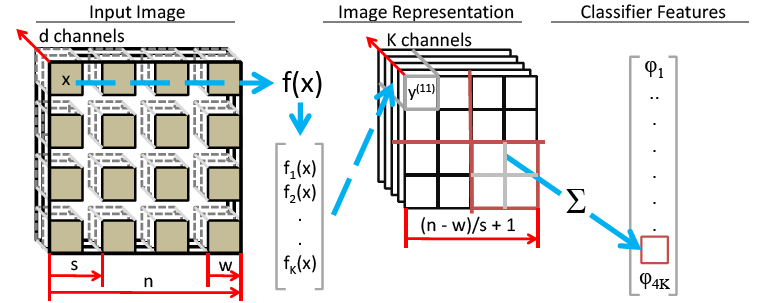
\includegraphics[width=\linewidth]{feature_extraction}
\caption{Feature 벡터 추출 과정 (Coates et al., 2011)}
\label{fig:feature_extraction}
\end{figure}

Feature 추출에 관련된 모든 작업을 다음과 같이 하나의 함수 $\Phi$로 표현해볼 수 있다.
\begin{align*}
    \Phi &\colon X \to [0, 1]^{6400} \\
    \Phi(\mathbf{x}) &= (\text{feature vector})
\end{align*}

\subsection{SVM 분류기}

$\Phi(X_{train})$을 입력으로 하고, $Y_{train}$을 출력으로 하여, SVM(L2) 분류기를 학습 시킨다.
이 학습한 분류기를 가지고 $\Phi(X_{test})$를 분류하게 된다.
본 실험에서는 선행 연구에서 구현한 SVM을 그대로 사용하였다.
SVM 자체에 대한 설명은 생략한다.

\section{추가 구현}

본 실험을 위해, 일단 Coates의 웹페이지에서 MATLAB으로 작성된 데모 코드를 얻었다.
데모 코드에는 앞 절에서 설명한 사항 외에 whitening 등 patch에 대한 normalization과 feature 벡터에 대한 standardization이 포함되어 있다.
여기에 코드를 추가하여 실험하였다.

\subsection{여러 soft한 K-means 알고리즘}

\ref{sec:feature_extractor}절을 주의 깊게 보면, 선행 연구에서 주목 할만한 점이 있다.
선행 연구 논문에서는 가장 가까운 중심점에 대한 activation만 1로 한 것을 K-means(hard)로, $\mathbf{f}$ 처럼 평균 이하를 버려서 activation을 바꿔준 것을 K-means(triangle)로 표기 하였다.
그리고 여러가지 무감독 학습(Auto-encoder, GMM 등) 중에 하나로 K-means(hard)와 K-means(triangle)을 구별하여 소개하였다.
그러나 이 부분은 misleading을 유발한다.
사실은 두 K-means 알고리즘이 중심점을 구하는 과정까지는 완벽히 동일함을 알 수 있다.
(E-M 알고리즘에서 responsibility를 1-of-N 대신 softmax 등의 확률을 사용하여 iteration을 도는) Soft K-means 알고리즘을 K-means(triangle) 알고리즘과 비교해볼 때 확연히 다르다.
다시 말하면, K-means(triangle)은 soft한 K-means 알고리즘이 아니다.
본 연구에서는 데모 코드를 보고 나서야, 이 부분을 misleading 했다고 알게 되었다.
결국 여러 soft한 K-means 알고리즘을 구현하여 비교하려던 초기 계획은 더이상 유효하지 않게 되었고, 따라서 진행할 수 없었다.

GMM은 대표적인 soft 클러스터링의 예로서 K-means를 일반화한 모델로 생각할 수 있다.
선행 연구에서 GMM을 사용했을 때의 성능이 K-means(hard)를 사용했을 때보다 더 낮게, 즉 가장 낮았다.
이 결과를 봤을 때 soft한 클러스터링 알고리즘을 사용하기 보다는 hard 클러스터링을 통해 먼저 중심점들을 구하고 난 이후에 activation을 어떻게 도출하는지가 성능 향상에 더 큰 영향을 미친다고 미루어 짐작할 수 있다.
Actication을 어떻게 계산하고 처리할 것인지는 pooling 단계의 일부로도 볼 수 있으므로, pooling에서 여러 실험을 수행 하였다.

\subsection{여러 pooling 방식}

\ref{sec:quadrant_pooling}절에서 사분면에 대한 sum pooling (SUM)에 대해 설명하였다.
이 외에 average pooling (AVG), max pooling (MAX), stochastic pooling (STOCH), stochastic max pooling (STOCHMAX)을 구현하였다.
이들도 마찬가지로 사분면에 대해 pooling 하도록 하였다.
부록에 MATLAB 구현을 첨부하였다.

\subsubsection{Average pooling (AVG)}

각 사분면에 대해 평균값을 구한다.
각 사분면의 크기가 13x13, 14x14 등으로 서로 달라서 feature 벡터를 standardization 하더라도 sum pooling과 결과가 다르다.
이렇게 하면 사분면 마다 standardization을 하는 효과가 있다.
Training 할 때와 testing 할 때 모두 같은 pooling 방식을 사용한다.

\subsubsection{Max pooling (MAX)}

각 사분면에 대해 최댓값을 구한다.
$K$개의 feature 각각에 대해 따로 적용한다.
Training 할 때와 testing 할 때 모두 같은 pooling 방식을 사용한다.

\subsubsection{Stochastic pooling (STOCH)}

Zeiler et al.(2013)의 연구에서 소개된 방식이다.
Training 할 때와 testing 할 때 서로 다른 pooling 방식을 사용한다.
Training 할 때에는, 각 사분면을 region이라고 할 때, activation들을 region에 속한 모든 activation의 합으로 나누어서 확률을 구한다.
그리고 한 region에서 이 확률에 따라 activation 중 하나를 고른다.
Testing 할 때에는, training 할 때와 같이 확률을 구하고 이 확률로 activation의 기댓값을 구한다.

기존 연구(ibid.)에서는 사분면으로 나누지 않았으며, region의 크기는 3x3이었다. MAX, AVG에 비해 더 좋은 성능을 내었다.

\subsubsection{Stochastic max pooling (STOCHMAX)}

Huang et al.(2015)의 연구에서 소개된 방식이다.
Training 할 때와 testing 할 때 서로 다른 pooling 방식을 사용한다.
Training 할 때에는, 각 사분면을 region이라고 할 때, region에 속한 activation들을 0.5의 확률로 버리고 남은 것 중에 최댓값을 고른다.
Testing 할 때에는, region에서 큰 activation부터 차례로 1/2, 1/4, 1/8의 가중치를 곱해 더한다.

기존 연구(ibid.)에서는 사분면으로 나누지 않았으며, region의 크기는 3x3이었다. STOCH 등에 비해 더 좋은 성능을 내었다.

\subsection{기타 구현}

선행 연구(Coates et al., 2011)에서는 CIFAR-10 데이터에 대한 분류 정확도에 \textbf{오차}가 나타나 있지 않다.
이 연구 결과를 검증하기 위해 SUM을 포함한 모든 pooling 방식에 대해 학습과 분류 전 과정을 \textbf{10번씩} 반복 실행하였다.
또한 testing 결과에 대한 \textbf{confusion matrix}를 출력하도록 하였다.
사소하지만 $imshow$로 되어 있던 구현을 $imwrite$로 변경하여 GUI 없이 실행 가능하게 하였으며, 실행 시간도 측정하였다.

\section{실험 결과}

\subsection{Pooling에 따른 정확도 비교}

각 pooling 방식에 따른 차이를 볼 수 있었다.
Training, testing에 대한 분류 정확도는 그림 \ref{fig:accuracy}와/과 같았고, testing에 대한 분류 정확도의 99\% 신뢰구간은 그림 \ref{fig:error_bar}와/과 같았다.

\begin{figure}[H]
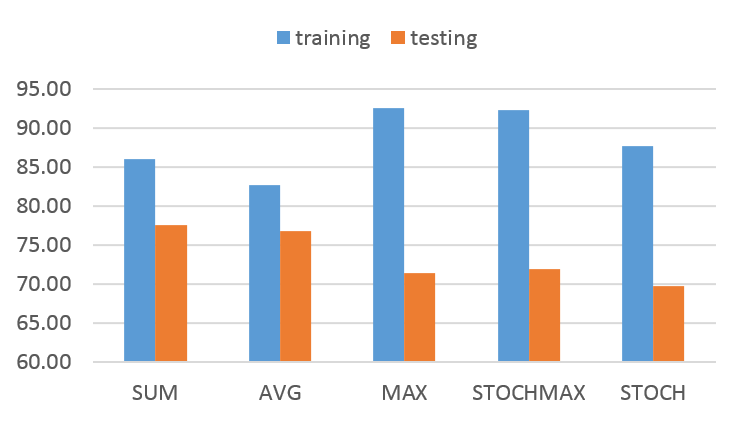
\includegraphics[width=\linewidth]{accuracy}
\caption{Pooling과 Train/Test 정확도(\%)}
\label{fig:accuracy}
\end{figure}

\begin{figure}[H]
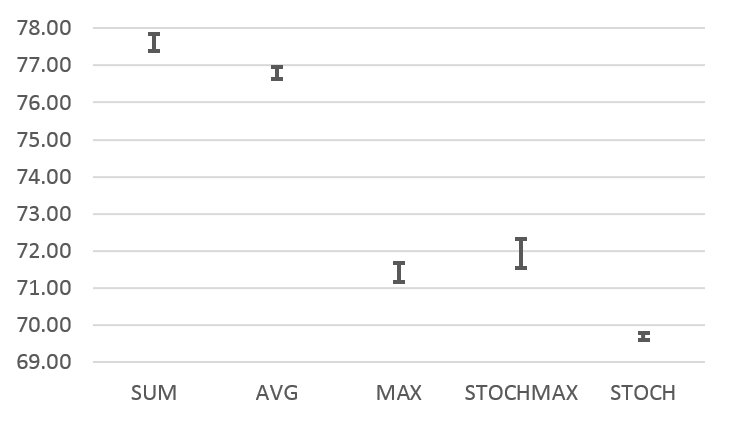
\includegraphics[width=\linewidth]{error_bar}
\caption{Pooling과 Test 정확도(\%) 99\% 신뢰구간}
\label{fig:error_bar}
\end{figure}

안타깝게도 모든 pooling 방식에 있어서 testing 분류 정확도가 기존의 SUM 방식을 넘지 못했다.
특히, AVG 방식의 경우 SUM에 비해 더 정밀한 standardization을 하게 되어 조금이라도 더 높은 성능을 얻을 수 있기를 기대했으나 그렇지 못했다.
SUM 방식의 정확도는 $77.61(\pm 0.23)$\%이었고, AVG 방식의 정확도는 $76.79(\pm 0.16)$\%이었다.
즉, 두 방식의 신뢰구간이 서로 완전히 분리되어 통계적으로 유의미하게 SUM 방식이 더 높은 성능을 보였다.
정밀한 standardization의 효과는 testing 분류 정확도의 향상으로 나타나는 대신 regularization에서 나타났다.
SUM 방식의 training 정확도와 testing 정확도의 차이는 $8.469$\%p인데 반해 AVG 방식은 $5.882$\%p 밖에 되지 않았다.
학습 과정에서 cross validation을 통해 하이퍼 파라미터를 조절하는 과정이 있다면, AVG 방식이 training 정확도와 testing 정확도의 차이가 적기 때문에 파라미터 조절에 있어서 testing 정확도를 높이는 방향을 예측 하기에 더 적합할 수 있을 것이다.

한가지 흥미로운 점은 선행 연구(2011)에서의 정확도(SUM 방식)는 $77.9$\%로서 신뢰구간의 상한 $77.84$\%를 약 $0.06$\%p 넘어서는 높은 성능을 냈다는 것이다.
유효 숫자를 맞추기 위해 선행 연구의 정확도의 유효 숫자를 한 자리 늘려서 가장 작은 값을 취한다 하더라도 $77.85$\%가 되는데 이 또한 신뢰구간의 상한 보다 $0.01$\%p 더 크다.
본 실험의 표본은 적은 편(10개)이기 때문에 단정 지을 수는 없지만, 선행 연구에서 높은 성능을 내기 위해 여러 번 수행하고 가장 높은 성능으로 표기하였을 가능성이 크다는 의심을 지울 수 없다.

MAX 방식과 SUM 방식을 비교하였을 때에는 MAX 방식의 경우는 overfitting이 아주 크게 나타남을 알 수 있다.
MAX 방식의 training 데이터에 대한 분류 정확도는 SUM 방식의 정확도 $86.082(\pm 0.067)$\%에 비해 압도적으로 높은 $92.655(\pm 0.088)$\%로 나타났지만, testing 데이터에 대한 분류 정확도는 $71.41(\pm 0.26)$\%으로 SUM 방식의 정확도에 비해 현저히 낮았다.
MAX 방식은 극단적인 값만 뽑는 pooling 방식이기 때문에 일반화를 잘 못한다고 해석할 수 있다.

STOCH 방식과 STOCHMAX 방식은 각각 Zeiler et al.(2013)의 연구와 Huang et al.(2015)의 연구에서 AVG, MAX 방식에 비해 높은 성능을 낸다고 자랑한 방식이다.
그러나 본 실험에서는 둘 다 SUM 방식에 비해 아주 낮은 성능을 보였다.
STOCH 방식의 testing 데이터에 대한 분류 정확도는 $69.69(\pm 0.09)$\%이었고, STOCHMAX 방식의 정확도는 $71.94(\pm 0.40)$\%이었다.
STOCHMAX 방식이 STOCH 방식에 비해 성능이 더 높게 나온 것은 기존 연구(2015)와 동일한 결과였다.
STOCHMAX 방식을 MAX 방식과 비교해보면 testing 정확도의 신뢰구간이 서로 겹쳐서 통계적으로 유의미한 차이는 없었다.
이 두 가지 새로운 pooling 방식이 본 실험에서 좋은 성능을 내지 못한 이유는 모델의 구조가 다르기 때문이라고 추측할 수 있다.
첫번째로, 본 실험은 선행 연구(2011)에서 정해놓은 하이퍼 파라미터를 그대로 사용하였는데 이 파라미터는 SUM 방식에 맞춰진 것이다.
두번째로, pooling을 적용한 region의 크기가 본 실험에서는 약 14x14로 두 기존 연구(2013, 2015)에서 한 region의 크기인 3x3에 비해 지나치게 크다.

\subsection{Confusion matrix}

\begin{figure}[H]
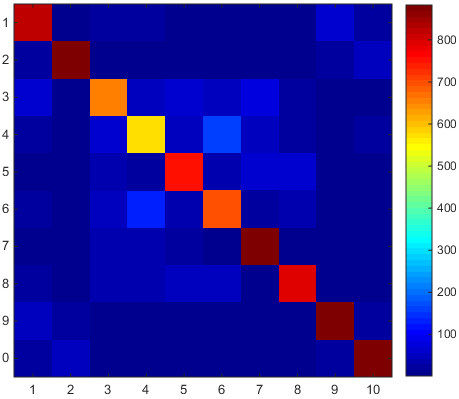
\includegraphics[width=\linewidth]{confusion_matrix}
\caption{분류 결과 Confusion Matrix 중 하나}
\label{fig:confusion_matrix}
\end{figure}

\begin{figure}[H]
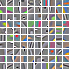
\includegraphics[width=\linewidth]{feature}
\caption{학습한 Feature 중 일부}
\label{fig:feature}
\end{figure}

SUM pooling 방식을 사용하여 가장 좋은 성능($77.88$\%)이 나온 결과에 대해 confusion matrix를 그려 보았다(그림 \ref{fig:confusion_matrix}).
(4, 4)와 (6, 6)이 흐리게 나온 것을 봤을 때 클래스 4와 6이 서로 헷갈리기 쉬움을 알 수 있었다.
클래스 4와 6은 각각 고양이와 개이다.
고양이와 개는 단순한 외형이 많이 닮아 있다.
본 실험에서는 convolution과 pooling을 한 번만 하여 단일 층 분류기를 구현했기 때문에 feature(6x6x3)들의 모습이 기껏해야 점이나 직선 정도의 복잡도를 가질 수 있다(그림 \ref{fig:feature}).
학습 층을 더 늘려서 곡선이나 원과 같은 복잡한 모양의 feature를 가질 수 있게 해야 고양이와 개를 더 정확히 구분할 수 있을 것이다.

\subsection{수행 시간 비교}

(TODO)

\section{결론}

각 pooling이 overfitting을 하는지 보고 논문의 결과에 대한 오차 분석을 하는 것이 목적
cross validation은 하지 않았다.
하이퍼 파라미터 때문인듯?
triangle k-means는 activation에 ReLU를 적용한 것과 사실상 같음

의의
오차 분석
표본이 적긴 하지만 선행 논문이 사기
misleading 지적

\section*{참고 문헌}

\begin{itemize}
\item Coates, A., Ng, A. Y., \& Lee, H. (2011). An analysis of single-layer networks in unsupervised feature learning. In \textit{International conference on artificial intelligence and statistics}.
\item Huang, Y., Sun, X., Lu, M., \& Xu, M. (2015). Channel-Max, Channel-Drop and Stochastic Max-Pooling. In \textit{Proceedings of the IEEE Conference on Computer Vision and Pattern Recognition Workshops}.
\item Zeiler, M. D., \& Fergus, R. (2013). Stochastic pooling for regularization of deep convolutional neural networks. \textit{arXiv preprint arXiv:1301.3557}.
\end{itemize}

\end{multicols*}

\pagebreak

\section*{부록}

\subsection*{실험 결과 표}

(TODO)

\subsection*{K-means 중심점}

(TODO)

\subsection*{추가한 pooling 코드}

\begin{lstlisting}
% pooling_sum.m
function XCi = pooling_sum(patches, prows, pcols)
  halfr = round(prows/2);
  halfc = round(pcols/2);
  q1 = sum(sum(patches(1:halfr, 1:halfc, :), 1),2);
  q2 = sum(sum(patches(halfr+1:end, 1:halfc, :), 1),2);
  q3 = sum(sum(patches(1:halfr, halfc+1:end, :), 1),2);
  q4 = sum(sum(patches(halfr+1:end, halfc+1:end, :), 1),2);
  XCi = [q1(:);q2(:);q3(:);q4(:)]';
end

% pooling_avg.m
function XCi = pooling_avg(patches, prows, pcols)
  halfr = round(prows/2);
  halfc = round(pcols/2);
  q1 = sum(sum(patches(1:halfr, 1:halfc, :), 1),2) ...
       / (halfr * halfc);
  q2 = sum(sum(patches(halfr+1:end, 1:halfc, :), 1),2) ...
       / ((prows - halfr) * halfc);
  q3 = sum(sum(patches(1:halfr, halfc+1:end, :), 1),2) ...
       / (halfr * (pcols - halfc));
  q4 = sum(sum(patches(halfr+1:end, halfc+1:end, :), 1),2) ...
       / ((prows - halfr) * (pcols - halfc));
  XCi = [q1(:);q2(:);q3(:);q4(:)]';
end

% pooling_max.m
function XCi = pooling_max(patches, prows, pcols)
  halfr = round(prows/2);
  halfc = round(pcols/2);
  q1 = max(max(patches(1:halfr, 1:halfc, :)),[],2);
  q2 = max(max(patches(halfr+1:end, 1:halfc, :)),[],2);
  q3 = max(max(patches(1:halfr, halfc+1:end, :)),[],2);
  q4 = max(max(patches(halfr+1:end, halfc+1:end, :)),[],2);
  XCi = [q1(:);q2(:);q3(:);q4(:)]';
end

% pooling_stochmax_train.m
function XCi = pooling_stochmax_train(patches, prows, pcols)
  function q = for_quad(sub)
    [r, c, z] = size(sub);
    sub = reshape(sub, 1, r * c, z);
    samp = rand(1, r * c, z) > 0.5;
    q = max(sub .* samp);
  end
  halfr = round(prows/2);
  halfc = round(pcols/2);
  q1 = for_quad(patches(1:halfr, 1:halfc, :));
  q2 = for_quad(patches(halfr+1:end, 1:halfc, :));
  q3 = for_quad(patches(1:halfr, halfc+1:end, :));
  q4 = for_quad(patches(halfr+1:end, halfc+1:end, :));
  XCi = [q1(:);q2(:);q3(:);q4(:)]';
end

% pooling_stochmax_test.m
function XCi = pooling_stochmax_test(patches, prows, pcols)
  function q = for_quad(sub)
    [r, c, z] = size(sub);
    prob = zeros(1, r * c);
    prob(1) = 1/2; prob(2) = 1/4; prob(3) = 1/8;
    sub = reshape(sub, 1, r * c, z);
    sorted = sort(sub, 'descend');
    q = sum(bsxfun(@times, sorted, prob));
  end
  halfr = round(prows/2);
  halfc = round(pcols/2);
  q1 = for_quad(patches(1:halfr, 1:halfc, :));
  q2 = for_quad(patches(halfr+1:end, 1:halfc, :));
  q3 = for_quad(patches(1:halfr, halfc+1:end, :));
  q4 = for_quad(patches(halfr+1:end, halfc+1:end, :));
  XCi = [q1(:);q2(:);q3(:);q4(:)]';
end

% pooling_stoch_train.m
function XCi = pooling_stoch_train(patches, prows, pcols)
  function q = for_quad(sub)
    [r, c, z] = size(sub);
    sub = reshape(sub, 1, r * c, z);
    sub_sum = sum(sub);
    sub_prob = bsxfun(@rdivide, sub, sub_sum);
    sub_prob = [zeros(1, 1, z) cumsum(sub_prob)];
    q = zeros(1, 1, z);
    for i = 1:z
      idx = sum(rand >= sub_prob(:, :, i));
      q(:, :, i) = sub(1, idx, i);
    end
  end
  halfr = round(prows/2);
  halfc = round(pcols/2);
  q1 = for_quad(patches(1:halfr, 1:halfc, :));
  q2 = for_quad(patches(halfr+1:end, 1:halfc, :));
  q3 = for_quad(patches(1:halfr, halfc+1:end, :));
  q4 = for_quad(patches(halfr+1:end, halfc+1:end, :));
  XCi = [q1(:);q2(:);q3(:);q4(:)]';
end

% pooling_stoch_test.m
function XCi = pooling_stoch_test(patches, prows, pcols)
  function q = for_quad(sub)
    bj = sum(sum(sub .^ 2, 1), 2);
    bm = sum(sum(sub, 1), 2);
    q = bj ./ bm;
    q(isnan(q)) = 0;
  end
  halfr = round(prows/2);
  halfc = round(pcols/2);
  q1 = for_quad(patches(1:halfr, 1:halfc, :));
  q2 = for_quad(patches(halfr+1:end, 1:halfc, :));
  q3 = for_quad(patches(1:halfr, halfc+1:end, :));
  q4 = for_quad(patches(halfr+1:end, halfc+1:end, :));
  XCi = [q1(:);q2(:);q3(:);q4(:)]';
end
\end{lstlisting}

\subsection*{코드 변경 사항 전체}

Github diff 링크: \url{https://goo.gl/qgUbqF}

변경 사항 통계(일부):
\begin{lstlisting}
    src/confusion_matrix.m         |   7 +
    src/extract_features.m         |  43 ++-
    src/kmeans_demo.m              |  69 +---
    src/minFunc/lbfgsC.mex         | Bin 0 -> 13080 bytes
    src/minFunc/mcholC.mex         | Bin 0 -> 21194 bytes
    src/pooling_avg.m              |   9 +
    src/pooling_max.m              |   9 +
    src/pooling_stoch_test.m       |  15 +
    src/pooling_stoch_train.m      |  21 ++
    src/pooling_stochmax_test.m    |  17 +
    src/pooling_stochmax_train.m   |  15 +
    src/pooling_sum.m              |   9 +
    src/run_classifier.m           |  58 ++++
    src/run_kmeans.m               |   2 +-
    src/show_centroids.m           |   2 -
    83 files changed, 416 insertions(+), 728 deletions(-)
\end{lstlisting}

\end{document}
